\documentclass[11pt,a4paper]{article}
\usepackage{gtu-el-yazisi}
\begin{document}
\notbilgi{Diferansiyel Denklemler}{4.--6. Hafta -- Fizik problemleri, varlık-teklik, Picard, Wronskiyen, sabit katsayılı denklemler}{dif-notu-part2-4-6-hafta.pdf}

\sayfa{1}
\section{Mekanik ve fizik problemlerinin Diferansiyel Denklemlere dönüştürülerek çözülmesi}

\[
  \text{$t$ anındaki değişim} = y'(t) = \lim_{\Delta t\to 0}\frac{y(t+\Delta t)-y(t)}{\Delta t}
\]

\subsection{(1) Newtonun ikinci kuralı:}
\[
  F = m\cdot a \qquad\qquad a = \frac{dV}{dt} \qquad\qquad V = \frac{dx}{dt}
\]

\subsection{(2) Oran problemleri (Radyoaktif parçalanma ve popülasyon)}
$t$ yıl sonra radyoaktif madde miktarı $x = x(t)$ olursa, onun parçalanma hızı $\dfrac{dx(t)}{dt}$ dir.

Parçalanma hızı, radyoaktif maddenin miktarı ile doğru orantılıdır yani:
\[
  \frac{dx}{dt} = -k\,x,\quad k>0 \qquad\qquad x(0)=x_0 \ \text{ile çözülür}
\]
{\small ($x$ $\rightarrow$ [parçalanmadan kalan madde miktarı])}

Popülasyon artımı için
\[
  \frac{dx}{dt} = k\,x,\quad k>0 \qquad\qquad x(0)=x_0
\]

\sayfa{2}
\subsection{(3) Karışım problemleri}

\begin{center}
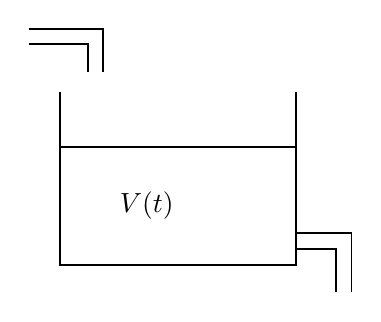
\begin{tikzpicture}[line width=0.7pt]
  % tank
  \draw (0,2.2) -- (0,0) -- (3,0) -- (3,2.2);
  \draw (0,1.5) -- (3,1.5);
  \node at (1.1,0.75) {$V(t)$};
  % giriş borusu (sol üst)
  \draw (-0.4,3.0) -- (0.55,3.0) -- (0.55,2.45);
  \draw (-0.4,2.8) -- (0.35,2.8) -- (0.35,2.45);
  % çıkış borusu (sağ alt)
  \draw (3,0.4) -- (3.7,0.4) -- (3.7,-0.35);
  \draw (3,0.2) -- (3.5,0.2) -- (3.5,-0.35);
\end{tikzpicture}
\end{center}

$V(t)$ $t$ anındaki karışımın hacmi\\
$x(t)$ $t$ anındaki tanktaki tuzun kütlesi\\
$C(t)$ konsantrasyon oranı $\displaystyle c(t)=\frac{x(t)}{V(t)}$
\[
  \frac{dx}{dt} = \text{rate in} - \text{rate out}
\]

Çözüm adımları
\begin{enumerate}[label=\arabic*.]
  \item birim zamanda giren tuzun miktarını hesaplarız
  \item herhangi bir anda kaptaki karışımın hacmini buluruz
  \item tuzun miktarını 2.\ de bulduğumuz hacime bölerek litre başına düşen tuzu buluruz
  \item hızla çarparak çıkan tuzu hesapla\okunamadi{rız}
\end{enumerate}

\sayfa{3}
\begin{enumerate}[label=\arabic*., start=5]
  \item sonra denklemi kurarız
  \[ \frac{dx}{dt} = \text{giren} - \text{çıkan} \]
  \item başlangıç koşulu $x_0$ belirlenir ve denklem çözülür
\end{enumerate}

\subsection{Soğuma Problemleri}
$T$ = cismin sıcaklığı

$T_e$ = onu çevreleyen ortamın sıcaklığı

Cismin sıcaklığının zamanla değişimin hızı
\[
  \frac{dT}{dt} = -k\,(T - T_e) \qquad k>0
\]

\sayfa{4}
\section{Varlık ve teklik}

\begin{tanim}
  $D\subset\mathbb{R}^2$ bölgesinde verilmiş $f(x,y)$ fonksiyonu $(x,y_1)$ ve $(x,y_2)\in D$ için
  \[
    \lvert f(x,y_1)-f(x,y_2)\rvert \le L\,\lvert y_1-y_2\rvert
  \]
  eşitsizliğini sağlayacak bir $L>0$ sabiti bulunursa, $f(x,y)$ $y$ değişkenine göre
  \textcolor{kirmizikalem}{Lipschitz} koşulunu sağlar. (tek)
\end{tanim}

\begin{teorem}
  \[
    \left\lvert \frac{\partial f}{\partial y}(x,y)\right\rvert \le L, \quad \forall (x,y)\in D \quad \text{sağlansın}
  \]
  O halde $f(x,y)$ fonksiyonu Lipschitz koşulunu sağlar.
\end{teorem}

\begin{teorem}[(Varlık ve teklik teoremi)]
  $f(x,y)$ \ $D$ bandından sürekli ise $\rightarrow$ çözüm var\\
  $f(x,y)$ \ $D$ \ \ '' \ \ $y$'ye göre lipschitz koşulunu sağlarsa $\rightarrow$ tek
\end{teorem}

\sayfa{5}
\section{Picard yaklaşımı}

\[
  \left.\begin{aligned}
    y' &= f(x,y)\\
    y(a) &= \alpha
  \end{aligned}\right\}
  \qquad
  \begin{aligned}
    y_0(x) &= \alpha\\
    y_n(x) &= \alpha + \int_a^x f\bigl(s, y_{n-1}(s)\bigr)\,ds
  \end{aligned}
\]

$n$. Picard yaklaşımının hata payı şu şekilde hesaplanır
\[
  \lvert y - y_n(x)\rvert \le M\cdot L^n\cdot \frac{h^{n+1}}{(n+1)!}
\]

$M$: $f(x,y)$ için üst sınır

$L$: Lipschitz sabiti

$h$: aralığın boyu

\sayfa{6}
\section{Wronskiyen nedir}

\[
  f(x),\ g(x) \;\longrightarrow\; W = \begin{vmatrix} f(x) & g(x)\\ f'(x) & g'(x) \end{vmatrix}
\]

$W = 0 \rightarrow f(x)$ ile $g(x)$ lineer bağımlı\\
$W \ne 0 \rightarrow f(x)$ \ \ '' \ \ '' \ \ '' \ \ bağımsız

\subsection{Abel's teoremi}
\[
  y'' + p(x)\,y' + q(x)\,y = 0 \qquad \text{2. dereceden homojen denklem}
\]
\[
  y_H = c_1\, y_1 + c_2\, y_2
\]
\[
  \text{\textcolor{kirmizikalem}{Abel's teoremi}} \;\rightarrow\; W(y_1,y_2) = c\cdot e^{-\int p(x)\,dx}
\]

\sayfa{7}
\section{2. derece sabit katsayılı homojen çözümündeki kurallar}

$\bigstar$\quad $y(x) = e^{kx} \;\Rightarrow\; y'(x) = k\,e^{kx} \;\Rightarrow\; y''(x) = k^2 e^{kx}$

\medskip
Karakteristik denklem oluşturma\\
$y'' + 2y' - 8y = 0$\,'nın karakteristik denklemi
\[
  k^2 + 2k - 8 = 0
\]
$r_1$ ve $r_2$ denklemin kökleri olmak üzere

\begin{enumerate}[label=\arabic*)]
  \item $\Delta > 0$ \quad $r_1 \ne r_2$ reel \qquad $y_H = c_1 e^{r_1 x} + c_2 e^{r_2 x}$
  \item $\Delta = 0$ \quad $r_1 = r_2$ reel \qquad $y_H = c_1 e^{r_1 x} + c_2\, x\, e^{r_2 x}$
  \item $\Delta < 0$ \quad $r_1 = a + bi$ \qquad $y_H = c_1 e^{ax}\cdot\cos(bx) + c_2 e^{ax}\sin(bx)$
\end{enumerate}

bu kurallar genişletilerek yüksek mertebeli homojen dif denklemlerde kullanılır

\end{document}
